\documentclass[12pt,a4paper]{article}
\usepackage[polish]{babel}
\usepackage[T1]{fontenc}
\usepackage[utf8x]{inputenc}
\usepackage{hyperref}
\usepackage{url}
\usepackage{graphicx}

\addtolength{\hoffset}{-1.5cm}
\addtolength{\marginparwidth}{-1.5cm}
\addtolength{\textwidth}{3cm}
\addtolength{\voffset}{-1cm}
\addtolength{\textheight}{2.5cm}
\setlength{\topmargin}{0cm}
\setlength{\headheight}{0cm}

\begin{document}

\title{Dokumentacja projektu ZPI}
\author{Dąbrowski Daniel\\ Gródek Damian\\ Jargut Piotr\\ Kocjan Katarzyna\\ Uryga Kamil}
\date{\today}

\maketitle

\begin{abstract}
Zarys dokumentacji projektowej stanowiący podstawę do realizacji projektu \\ zespołowego. 
\end{abstract}



\newpage

\tableofcontents
\listoffigures



\newpage

\section{Tytuł: System wspomagający szybkie parkowanie}

\section{Nazwa robocza: Parkingowy}

\section{Cel}
\begin{quotation}
Zoptymalizować ruch na parkingach i zniwelować długi czas szukania miejsca parkingowego, co pozwoli na zmniejszenie emisji spalin do atmosfery.
\end{quotation}
\begin{quotation}
Przewidywany termin ukończenia projektu 10 Maja.
\end{quotation}

\section{Zakres}

\subsection{Analiza wymagań}

{\large \bf System:}
\begin{itemize}
\item Określenie optymalnego rozmieszczenia emiterów beacon na podstawie planu parkingu;
\item Instalacja brokera MQTT i serwera node red;
\item Implementacja komunikacji pomiędzy czujnikami zajętości miejsca a brokerem MQTT;
\item Stworzenie bazy danych MSSQL;
\item Implementacja zapisu statusu czujników do bazy danych za pośrednictwem serwera node-red;
\item Implementacja wyzwalacza funkcji MSSQL przeliczającej ilość wolnych miejsc w danych sektorach w przypadku zmiany statusu któregokolwiek z czujników;
\item Implementacja odczytu ilości wolnych miejsc w danych sektorach po zmianie statusu któregokolwiek z czujników;
\item Wysłanie informacji do monitorów znajdujących się na węzłach komunikacyjnych.\\Monitory wyświetlają ilość wolnych miejsc w danym sektorze;
\item Implementacja komunikacji pomiędzy skanerami przy szlabanach a serwerem.
\end{itemize}
{\large \bf Użytkownik :}

{\bf Aplikacja mobilna:}
\begin{itemize}
\item System lokalizacji;
\item System rejestracji;
\item System logowania do aplikacji;
\item Gotowy system.
\end{itemize}

{\bf System wspomagający parkowanie:}
\begin{itemize}
\item System zarządzający wolnymi miejscami;
\item System sygnałów świetlnych.
\end{itemize}

{\bf System lokalizacji pojazdu na parkingu:}
\begin{itemize}
\item System nawigacji do samochodu;
\item Zapamiętanie lokalizacji samochodu.
\end{itemize}
{\large \bf Administrator:}
\begin{itemize}
\item Gotowe rozmieszczenie urządzeń/sprzętu;
\item Gotowe rozmieszczenie czujników;
\item Gotowe połączenia bezprzewodowe z urządzeniami i serwerem na celu serwisu i identyfikacji wymiany baterii bądź naprawy czujników.
\end{itemize}

\subsection{Wymagania funkcjonalne i niefunkcjonalne}
{\large \bf Wymagania funkcjonalne:}
\begin{itemize}
\item Czujnik zajętości miejsca umieszczony w nawierzchni wysyła sygnał ultradźwiękowy, na podstawie czasu powrotu sygnału odbitego określa odległość do przeszkody. Odległość 0-40cm uznawana jest jako zajęte miejsce;
\item Czujnik łączy się z brokerem MQTT wysyłając swoje id, status i stan naładowania baterii. Na serwerze node red Blok MQTT połączony z odpowiednim topic’iem\\w  brokerze odbiera dane zajętości miejsca. Wysyła je do bloku funkcji, funkcja bazując na danych wejściowych wybiera odpowiednią procedurę modyfikującą status czujnika\\w bazie danych MSSQL. Funkcja wysyła procedurę do bloku MSSQL;
\item Czujnik zajętości miejsca powinien wysyłać stan baterii do serwera MSSQL w przypadku kiedy poziom naładowania baterii spadnie poniżej 10\%;
\item Administrator za pomocą aplikacji webowej powinien mieć wgląd na status czujników zajętości i ich poziom naładowania baterii;
\item Serwer MSSQL powinien przeliczać ilość wolnych miejsc w momencie odebrania\\informacji o zmianie statusu któregokolwiek z nich;
\item Aplikacja mobilna powinna wyświetlać aktualna informacje o ilości wolnych miejsc, która jest na bieżąco aktualizowana z bazy danych MSSQL w momencie ponownego przeliczenia wolnych miejsc;
\item Zmiana statusu zajętości któregokolwiek z miejsc spowoduje wywołanie funkcji\\obliczającej zajętość miejsc w danych sektorach bądź piętrach. Za pomocą protokołu MQTT wysłana zostanie informacja do sterownika WEMOS, który wyświetli ilość\\wolnych miejsc na tablicy znajdującej się w pobliżu węzłów komunikacyjnych;
\item Aplikacja mobilna, za pomocą triangulacji, będzie wyznaczać aktualną pozycję pojazdu w przestrzeni dwuwymiarowej względem nadajników beacon;
\item Aplikacja mobilna zapewni możliwość zapisania w bazie danych aktualnej lokalizacji samocho użytkownika poprzez wybranie odpowiedniej opcji, co umożliwi zlokalizowanie zaparkowanego samochodu;
\item Aplikacja mobilna poprzez wybór opcji znalezienia samochodu, pobierze koordynaty zaparkowanego samochodu z bazy danych oraz wyznaczy aktualną pozycję użytkownika. Aplikacja wyświetla położenie użytkownika i jego samochodu;
\item Aplikacja mobilna, na podstawie id użytkownika, wygeneruje unikalny kod QR,\\za pomocą którego rejestrowany będzie wjazd oraz wyjazd z parkingu;
\item Skaner za pomocą transmisji szeregowej wyśle identyfikator użytkownika do bloku serial na serwerze node-red. Zostanie wywołana funkcja z procedurą SQL zmieniającą status użytkownika oraz zapisującą aktualną datę i godzinę wjazdu i wyjazdu;
\item System umożliwi użytkownikom rejestrację oraz logowanie do aplikacji mobilnej.
\end{itemize}
{\large \bf Wymagania niefunkcjonalne:}
\begin{itemize}
\item Aplikacja powinna być darmowa;
\item Aplikacja powinna mieć intuicyjny i przejrzysty interfejs;
\item Aplikacja powinna być kompatybilna z większością urządzeń aby mogło używać jej jak najwięcej użytkowników.
\end{itemize}



\newpage

\subsection{Diagram przypadków użycia i diagram przepływu (opcjonalny)}
\begin{figure}[htb!p]
\begin{center}
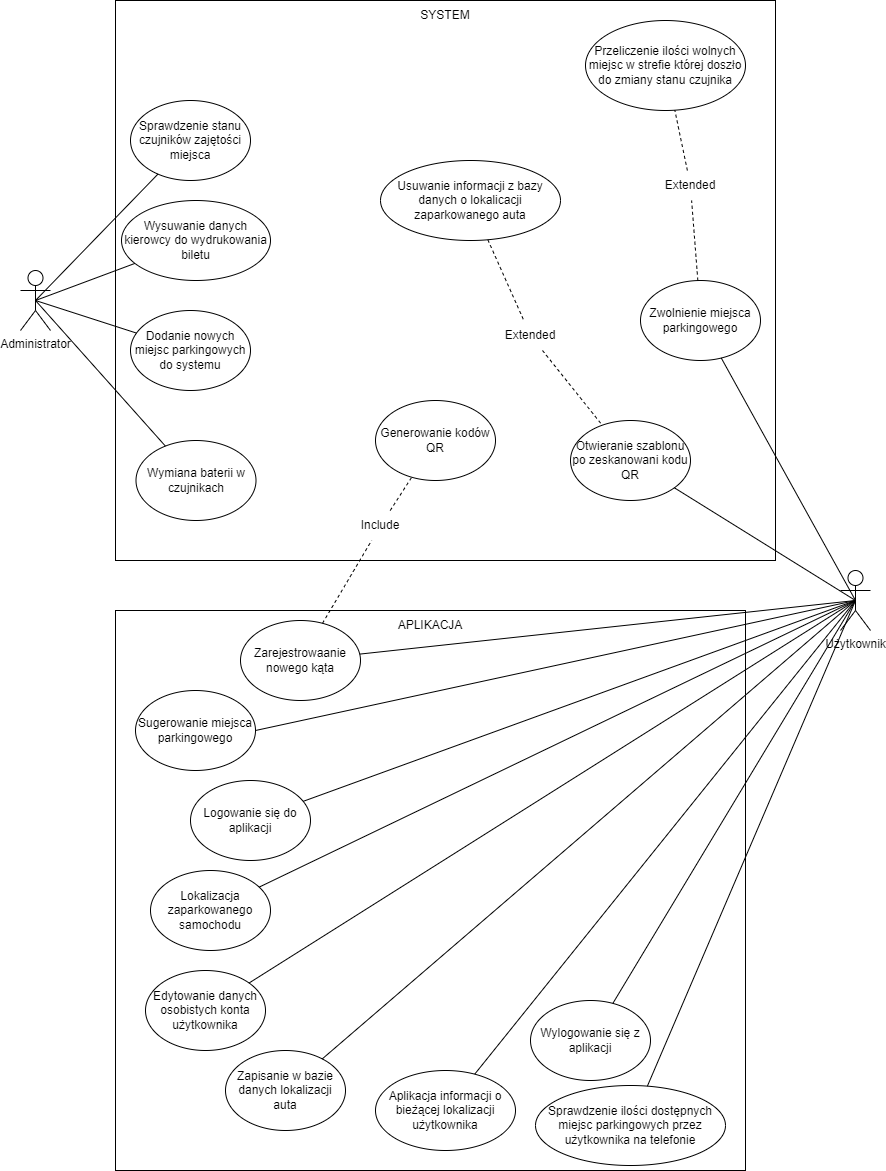
\includegraphics[width=0.9\textwidth]{Untitled Diagram.drawio.png}
\caption{Diagram przypadków użycia}
\end{center}
\end{figure}

\subsection{Dobór technologii}
\begin{itemize}
\item Emitery beacon pracujące na protokole BT low energy (Access pointy zintegrowane z emiterami Beacon);
\item Ultradźwiękowe czujniki zajętości miejsca (Wi-Fi, MQTT);
\item Wyświetlacze;
\item Sterowniki do wyświetlaczy (Wemos D1);
\item Windows;
\item Broker MQTT (RabitMQTT, Mosquito);
\item Android Studio(język JAVA);
\item Node-RED;
\item MSSQL;
\item ASP NET 4.8  (C\#);
\item DevExpress 20.1.6.
\end{itemize}

\section{Scenariusze}
{\large \bf Scenariusz:} Sugerowanie miejsca parkingowego
\\{\bf Nr:} 01
\\{\bf Aktor:} Użytkownik aplikacji mobilnej
\\{\bf Stan wejścia:}

Warunek: Posiadanie aplikacji, znalezienie się przy wjeździe do parkingu.
\\{\bf Przebieg scenariusza:}
\begin{enumerate}
\item Użytkownik rejestruje wjazd na parking skanując kod QR aplikacji przy szlabanie,\\informacja zawierająca ID użytkownika przekazywana jest portem szeregowym\\do serwera. W bazie danych zmieniany jest status użytkownika;
\item Użytkownik obserwuje monitory znajdujące się na węzłach komunikacyjnych\\informujące o ilości wolnych miejsc w najbliższym sektorze;
\item Użytkownik parkuje samochód  na odpowiadającym mu miejscu. Czujnik zajętości\\rejestruje zajęcie miejsca parkingowego, wysyła informację o zmianie statusu miejsca\\na “zajęte” do serwera.
\end{enumerate}
{\bf Wynik:} Użytkownik bez problemu parkuje swój pojazd i zmieniony zostaje status\\użytkownika.
\newline\newline\newline\newline
{\large \bf Scenariusz:} Zwolnienie miejsca parkingowego
\\{\bf Nr:} 02
\\{\bf Aktor:} Użytkownik aplikacji mobilnej
\\{\bf Stan wejścia:}

Warunek: Użytkownik ma już zaparkowane auto na parkingu.
\\{\bf Przebieg scenariusza:}
\begin{enumerate}
\item Użytkownik opuszcza miejsce parkingowe;
\item Czujnik zajętości rejestruje opuszczenie miejsca parkingowego, wysyła informację o zmianie statusu miejsca na “wolne” do serwera;
\item Użytkownik rejestruje wyjazd z parkingu. Informacja zawierająca Id użytkownika jest przekazywana portem szeregowym do serwera. Wprowadzana jest zmiana statusu użytkownika w bazie danych oraz zerowana jest zapisana lokalizacja samochodu.
\end{enumerate}
{\bf Wynik:} Użytkownik opuszcza parking.
\newline\newline
{\large \bf Scenariusz:} Lokalizacja zaparkowanego samochodu
\\{\bf Nr:} 03
\\{\bf Aktor:} Użytkownik aplikacji mobilnej
\\{\bf Stan wejścia:}

Warunek: Użytkownik ma już zaparkowane auto na parkingu oraz ma zainstalowaną \\aplikację i zapisał w aplikacji miejsce w którym zaparkował.
\\{\bf Przebieg scenariusza:}
\begin{enumerate}
\item Użytkownik wraca np. z zakupów i zapomniał gdzie zaparkował;
\item Aplikacja pokazuje miejsce gdzie auto zostało zaparkowane i obecną lokalizację\\Użytkownika;
\item Użytkownik znajduje swój pojazd i wyjeżdza z parkingu.
\end{enumerate}
{\bf Scenariusz alternatywny:}
\begin{enumerate}
\item Użytkownik nie zapisał pkt parkowania przez co aplikacja nie pokazuje lokalizacji;
\item Użytkownik jest zmuszony szukać swojego samochodu  bo nie zapisał lokalizacji gdzie zaparkował.
\end{enumerate}
{\bf Wynik:} Użytkownik znajduje swój pojazd i opuszcza parking.
\newline\newline\newline\newline\newline\newline\newline\newline\newline
{\large \bf Scenariusz:} Rozładowanie telefonu
\\{\bf Nr:} 04
\\{\bf Aktor:} Użytkownik aplikacji mobilnej
\\{\bf Stan wejścia:}

Warunek: Użytkownik ma już zaparkowane auto na parkingu.
\\{\bf Przebieg scenariusza:}
\begin{enumerate}
\item Jeśli w czasie np. zakupów użytkownikowi rozładuje się telefon nie będzie on w stanie wyjechać;
\item Jeśli nie jest sam może on zalogowac sie z innego telefonu(osoby towarzyszącej);
\item Użytkownik loguje się z innego telefonu pobiera aplikacje;
\item Po wpisaniu danych do aplikacji loguje się i może wyjechać.
\end{enumerate}
{\bf Scenariusz alternatywny 1:}
\begin{enumerate}
\item Jeżeli osoba jest sama i jeśli posiada ładowarke samochodową ładuje telefon aby móc uruchomić aplikację;
\item Użytkownik wyjeżdza z parkingu.
\end{enumerate}
{\bf Scenariusz alternatywny 2:}
\begin{enumerate}
\item Użytkownik nie posiada ładowarki samochodowej;
\item Użytkownik idzie do budki ochroniarskiej i przekazuje swoje dane do identyfikacji;
\item Użytkownik dostaje bilecik dzięki któremu wyjedzie;
\item Użytkownik wyjeżdża z parkingu.
\end{enumerate}
{\bf Wynik:} Użytkownik ponownie uzyskuje dostęp do aplikacji / dostaje bilet z kodem QR\\i opuszcza parking.
\newline\newline\newline\newline\newline\newline\newline\newline\newline\newline\newline\newline\newline\newline\newline\newline
{\large \bf Scenariusz:} Wymiana baterii w czujnikach
\\{\bf Nr:} 05
\\{\bf Aktor:} Administrator
\\{\bf Stan wejścia:}

Warunek: Rozładowanie baterii w czujnikach.
\\{\bf Przebieg scenariusza:}
\begin{enumerate}
\item Czujniki na bieżąco wysyłają informacje o stanie baterii do serwera;
\item Administrator odczytuje w aplikacji web poziom naładowania baterii;
\item Administrator wymienia w wymaganych czujnikach baterie.
\end{enumerate}
{\bf Wynik:} Czujniki działają dalej sprawnie dzięki wymienionym bateriom.
\newline\newline
{\large \bf Scenariusz:} Dodanie nowych miejsc parkingowych do systemu
\\{\bf Nr:} 06
\\{\bf Aktor:} Administrator
\\{\bf Stan wejścia:}

Warunek: Rozbudowa o nowe miejsca parkingowe.
\\{\bf Przebieg scenariusza:}
\begin{enumerate}
\item Administrator konfiguruje nowe czujniki i odczytuje UID;
\item Administrator dodaje czujniki do do bazy danych, konfiguruje połączenie MQTT\\z brokerem, dodaje nowe bloki do node red’a i tworzy zapytania SQL;
\item Administrator zaleca programistom zaktualizowanie aplikacji o nowe miejsca\\parkingowe.
\end{enumerate}
{\bf Wynik:} Aplikacja została zaktualizowana, a baza danych zwiększona o nowe rekordy.
\newline\newline
{\large \bf Scenariusz:} Generowanie kodu QR dla użytkownika
\\{\bf Nr:} 07
\\{\bf Aktor:} Użytkownik aplikacji mobilnej
\\{\bf Stan wejścia:}

Warunek: Tworzenie nowego konta przez użytkownika.
\\{\bf Przebieg scenariusza:}
\begin{enumerate}
\item Użytkownik wpisuje swoje dane;
\item Aplikacja mobilna generuje kod QR  na podstawie UUID użytkownika wygenerowanego w bazie danych podczas tworzenia konta.
\end{enumerate}
{\bf Wynik:} Aplikacja generuje kod QR.
\newline\newline\newline\newline\newline
{\large \bf Scenariusz:} Logowanie się do aplikacji
\\{\bf Nr:} 08
\\{\bf Aktor:} Użytkownik aplikacji mobilnej / webowej
\\{\bf Stan wejścia:}

Warunek: Użytkownik posiada już zarejestrowane konto.
\\{\bf Przebieg scenariusza:}
\begin{enumerate}
\item Użytkownik wybiera opcję logowania;
\item Wpisuje dane logowania;
\item System logowania komunikuje się z bazą danych w celu weryfikacji danych;
\item System logowania otrzymuje potwierdzenie poprawności danych;
\item System logowania przenosi Użytkownika na główną stronę dla zalogowanych.
\end{enumerate}
{\bf Scenariusz alternatywny:}
\begin{enumerate}
\item Użytkownik podał błędne dane logowania / zostawił puste pole;
\item Aplikacja informuje o nieprawidłowych danych i prosi o nie jeszcze raz.
\end{enumerate}
{\bf Wynik:} Użytkownik loguje się do aplikacji mobilnej / webowej.
\newline\newline
{\large \bf Scenariusz:} Wylogowanie się z aplikacji
\\{\bf Nr:} 09
\\{\bf Aktor:} Użytkownik aplikacji mobilnej / webowej
\\{\bf Stan wejścia:}

Warunek: Użytkownik posiada już zarejestrowane konto.
\\{\bf Przebieg scenariusza:}
\begin{enumerate}
\item Użytkownik włącza aplikacje i przechodzi do ustawień gdzie wybiera opcje wylogowania;
\item Użytkownik po wylogowaniu może ponownie się zalogować.
\end{enumerate}
{\bf Wynik:} Użytkownik wylogował się z aplikacji mobilnej / webowej.
\newline\newline\newline\newline\newline\newline\newline\newline\newline\newline\newline\newline\newline\newline
{\large \bf Scenariusz:} Zarejestrowanie nowego konta
\\{\bf Nr:} 10
\\{\bf Aktor:} Użytkownik aplikacji mobilnej
\\{\bf Stan wejścia:}

Warunek: Użytkownik ma zainstalowaną aplikacje.
\\{\bf Przebieg scenariusza:}
\begin{enumerate}
\item Użytkownik wprowadza dane osobiste wymagane do utworzenia nowego konta\\(login, hasło, imię, nazwisko, adres, e-mail, nr. telefonu);
\item Wygenerowanie nowego kodu QR (scenariusz 7);
\item Aktualizacja bazy użytkowników.
\end{enumerate}
{\bf Wynik:} Użytkownik ma utworzone nowe konto do korzystania z aplikacji mobilnej.
\newline\newline
{\large \bf Scenariusz:} Edytowanie danych osobistych konta użytkownika
\\{\bf Nr:} 11
\\{\bf Aktor:} Użytkownik aplikacji mobilnej / webowej
\\{\bf Stan wejścia:}

Warunek: Dane użytkownika nie są już aktualne.
\\{\bf Przebieg scenariusza:}
\begin{enumerate}
\item Użytkownik wybiera opcję edytowania danych konta;
\item Aplikacja mobilna / webowa pobiera dane z bazy danych;
\item Użytkownik wpisuje aktualne dane osobiste;
\item Po zatwierdzeniu przez użytkownika poprawności danych baza danych zostanie\\zaktualizowana.
\end{enumerate}
{\bf Scenariusz alternatywny:}
\begin{enumerate}
\item Użytkownik podał błędne dane / zostawił puste pole;
\item Aplikacja informuje o nieprawidłowych danych i prosi o nie jeszcze raz.
\end{enumerate}
{\bf Wynik:} Użytkownik aktualizuje dane w aplikacji mobilnej / webowej.
\newline\newline\newline\newline\newline\newline\newline\newline\newline\newline\newline\newline
{\large \bf Scenariusz:} Otwieranie szlabanu po zeskanowaniu kodu QR
\\{\bf Nr:} 12
\\{\bf Aktor:} Użytkownik aplikacji mobilnej
\\{\bf Stan wejścia:}

Warunek: Posiadanie aplikacji mobilnej.
\\{\bf Przebieg scenariusza:}
\begin{enumerate}
\item Użytkownik podjeżdża pod szlaban otwiera aplikację mobilną;
\item Przybliża telefon do czujnika gdzie jest skanowany kod QR;
\item Po zeskanowaniu kodu szlaban zostaje podniesiony.
\end{enumerate}
{\bf Wynik:} Użytkownik wjeżdża / wyjeżdża z parkingu.
\newline\newline
{\large \bf Scenariusz:} Przeliczenie ilości wolnych miejsc w strefie której doszło do zmiany stanu czujnika
\\{\bf Nr:} 13
\\{\bf Aktor:} Użytkownik aplikacji mobilnej
\\{\bf Stan wejścia:}

Warunek: Użytkownik wjeżdża lub odjeżdża z miejsca parkingowego.
\\{\bf Przebieg scenariusza:}
\begin{enumerate}
\item Czujnik wysyła do serwera status zajętości;
\item Serwer po otrzymaniu informacji inicjuje funkcję wysyłając zapytanie do serwera.\\Zapytanie mające przeliczyć ilość wolnych miejsc zgodnie z sektorem, w którym znajduje się czujnik;
\item Zapisanie ilości wolnych miejsc zgodnie z sektorem w którym doszło do zmiany;
\item Baz danych zwraca ilość wolnych miejsc w danym sektorze. Serwer wysyła informację o ilości wolnych miejsc do sterownika monitora znajdującego się w danym sektorze.
\end{enumerate}
{\bf Wynik:} Pomyślnie zostanie zaktualizowana baza zajętości miejsc oraz monitory\\wyświetlające ilość wolnych miejsc.
\newline\newline\newline\newline\newline\newline\newline\newline\newline\newline\newline\newline\newline\newline
{\large \bf Scenariusz:} Zapisanie w bazie danych lokalizacji auta (Triangulacja)
\\{\bf Nr:} 14
\\{\bf Aktor:} Użytkownik aplikacji mobilnej
\\{\bf Stan wejścia:}

Warunek: Wybranie opcji zapisania lokalizacji pojazdu.
\\{\bf Przebieg scenariusza:}
\begin{enumerate}
\item Aplikacja mobilna pobiera dane odległości z 3 najbliższych beaconów;
\item Przy użyciu triangulacji i pobranych danych zostaje wyliczona przybliżona obecna\\lokalizacja telefonu (pojazdu);
\item Aplikacja przypisuje do danych użytkownika lokalizacje telefonu.
\end{enumerate}
{\bf Wynik:} Zostaje zapisana lokalizacja telefonu (pojazdu) w bazie danych.
\newline\newline
{\large \bf Scenariusz:} Aktualizacja informacji o bieżącej lokalizacji użytkownika
\\{\bf Nr:} 15
\\{\bf Aktor:} Użytkownik aplikacji mobilnej
\\{\bf Stan wejścia:}

Warunek: Uruchomienie aplikacji, znajdowanie się na obszarze parkingu.
\\{\bf Przebieg scenariusza:}
\begin{enumerate}
\item Aplikacja mobilna pobiera dane odległości z 3 najbliższych beaconów;
\item Przy użyciu triangulacji i pobranych danych zostaje wyliczona obecna lokalizacja\\telefonu (użytkownika);
\item Aplikacja mobilna wyświetla na mapie obecną lokalizację.
\end{enumerate}
{\bf Wynik:} Wyświetlanie obecnej lokalizacji.
\newline\newline
{\large \bf Scenariusz:} Usuwanie informacji z bazy danych o lokalizacji zaparkowanego auta\\(po opuszczeniu parkingu)
\\{\bf Nr:} 16
\\{\bf Aktor:} Użytkownik aplikacji mobilnej
\\{\bf Stan wejścia:}

Warunek: Zeskanowanie kodu QR na wyjeździe.
\\{\bf Przebieg scenariusza:}
\begin{enumerate}
\item Użytkownik opuszcza parking;
\item Skaner wysyła identyfikator użytkownika do serwera;
\item Na podstawie identyfikatora użytkownika usuwane zostają tymczasowe dane z bazy\\danych i zmieniony zostaje status użytkownika.
\end{enumerate}
{\bf Wynik:} Z bazy danych usuwane zostają tymczasowe dane użytkownika (lokalizacja\\zaparkowanego pojazdu) i zmieniony zostaje status użytkownika.
\newline\newline
{\large \bf Scenariusz:} Wyszukanie danych kierowcy do wydrukowania biletu (kodu QR\\użytkownika)
\\{\bf Nr:} 17
\\{\bf Aktor:} Administrator
\\{\bf Stan wejścia:}

Warunek: Użytkownik stracił dostęp do aplikacji mobilnej i nie może opuścić parkingu.
\\{\bf Przebieg scenariusza:}
\begin{enumerate}
\item Administrator na podstawie danych do identyfikacji od użytkownika szuka jego rekordu w bazie danych;
\item Administrator drukuje bilet z unikalnym kodem QR użytkownika.
\end{enumerate}
{\bf Wynik:} Użytkownik otrzymuje bilet z kodem QR do opuszczenia parkingu.
\newline\newline
{\large \bf Scenariusz:} Sprawdzenie ilości dostępnych miejsc parkingowych przez użytkownika\\na telefonie
\\{\bf Nr:} 18
\\{\bf Aktor:} Użytkownik aplikacji mobilnej
\\{\bf Stan wejścia:}

Warunek: Posiadanie Aplikacji .
\\{\bf Przebieg scenariusza:}
\begin{enumerate}
\item Użytkownik otwiera aplikację w celu sprawdzenia ilości miejsc na parkingu na danym piętrze;
\item Aplikacja mobilna pobiera dane z bazy danych i wyświetla informacje o wolnych miejscach w strefach na danym piętrze.
\end{enumerate}
{\bf Wynik:} Użytkownik otrzymuje informacje o ilości wolnych miejsc na danym piętrze.
\newline\newline
{\large \bf Scenariusz:} Sprawdzenie stanu czujników zajętości miejsca
\\{\bf Nr:} 19
\\{\bf Aktor:} Administrator
\\{\bf Stan wejścia:}

Warunek: Zepsuty czujnik zajętości miejsca.
\\{\bf Przebieg scenariusza:}
\begin{enumerate}
\item Czujniki wysyłają regularnie informacje o poprawnym działaniu;
\item Administrator sprawdza na aplikacji webowej stan działania czujników;
\item Administrator wymienia czujniki które przestały wysyłać informacje o poprawnym działaniu;
\item Administrator koryguje dane czujnika w bazie danych zgodnie z schematem.
\end{enumerate}
{\bf Wynik:} Wszystkie czujniki działają poprawnie.



\newpage

\section{Estymacja czasowa}
\begin{figure}[htb!p]
\begin{center}
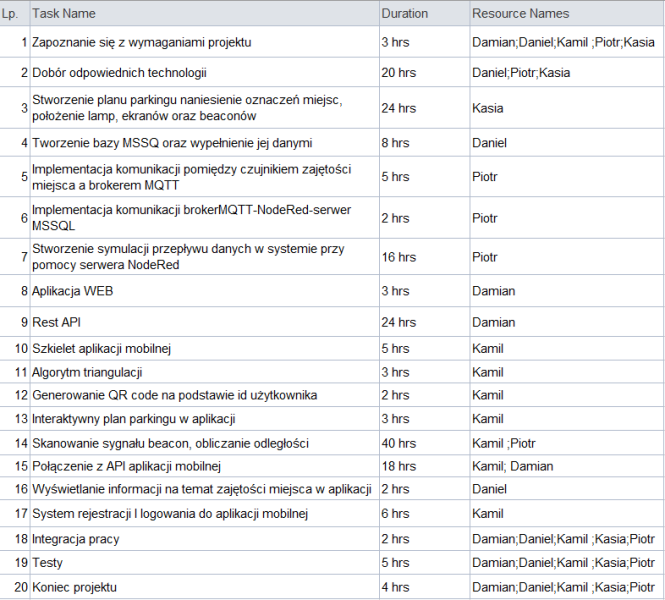
\includegraphics[width=0.9\textwidth]{unknown2.png}
\caption{Estymacja czasowa}
\end{center}
\end{figure}

\section{Implementacja}
\ \ \ \ \ \ Implementacja  symulacji pracy czujników zajętości miejsca przy pomocy Node -Red i Brokera MQTT. Symulacja  pokazuje przepływ informacji oraz zapis do bazy danych na podstawie danych otrzymanych z czujnika. Zasymulowany został również  przepływ informacji pomiędzy  serwerem mssql a kontrolerami oświetlenia sygnalizacyjnego oraz ekranami wyświetlającymi ilość wolnych miejsc.

Aplikacja Web napisana przy użyciu ASP.NET z biblioteką DevExpress, wykorzystywana do wyświetlania listy miejsc parkingowych, wstawiania nowych, oraz poziomu naładowania czujników zajętości miejsca. Strona pozwala również na sprawdzenie historii zajmowania miejsc parkingowych oraz sprawdzić listę beaconów i wprowadzić nowe beacony do bazy.

Rest API - Wykonany w Node.JS, pozwala na komunikację aplikacji mobilnej z serwerem SQL. Za pomocą tokenów JSON Web Token jest wykonywana autoryzacja użytkownika, po 5 minutach token jest unieważniany.

Aplikacja Mobilna - Łączy się z serwerem Rest API w Node.JS. Pozwala na zarejestrowanie użytkownika, zalogowanie się, pobranie ile jest wolnych miejsc na parkingu. Wykorzystywana jest do zarejestrowania kiedy użytkownik wjechał na parking, na zapisanie gdzie zaparkowany jest samochód i zapisanie kiedy użytkownik wyjechał z parkingu.

Aplikacja łączy się z beaconami w celu ustalenia lokacji użytkownika i samochodu.

Projekt dwóch pięter parkingu z miejscami parkingowymi.

%\begin{figure}[htb!p]
%\begin{center}
%\includegraphics[width=0.9\textwidth]{piętro_0.png}
%\caption{Piętro 0}
%\end{center}
%\end{figure}

%\begin{figure}[htb!p]
%\begin{center}
%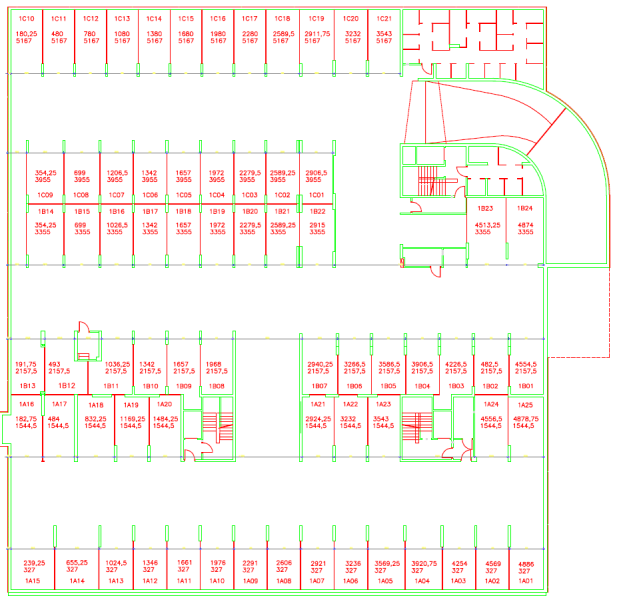
\includegraphics[width=0.9\textwidth]{piętro_-1.png}
%\caption{Piętro -1}
%\end{center}
%\end{figure}

Beacony naniesione na plan parkingu.

\begin{figure}[htb!p]
\begin{center}
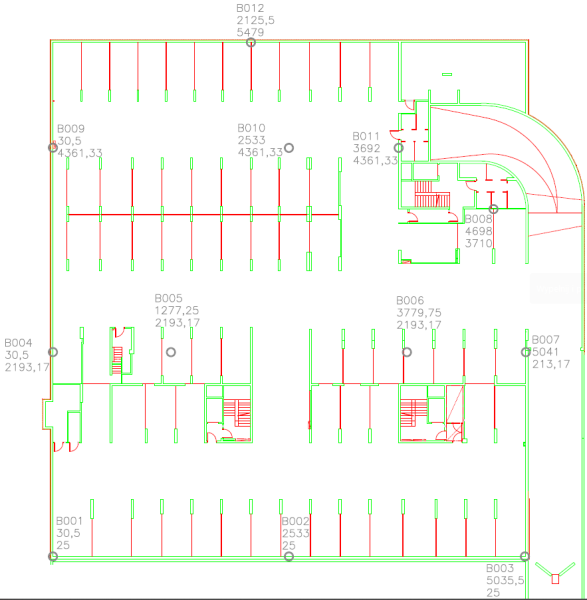
\includegraphics[width=0.9\textwidth]{beacon_0.png}
\caption{Beacony piętro 0}
\end{center}
\end{figure}

\begin{figure}[htb!p]
\begin{center}
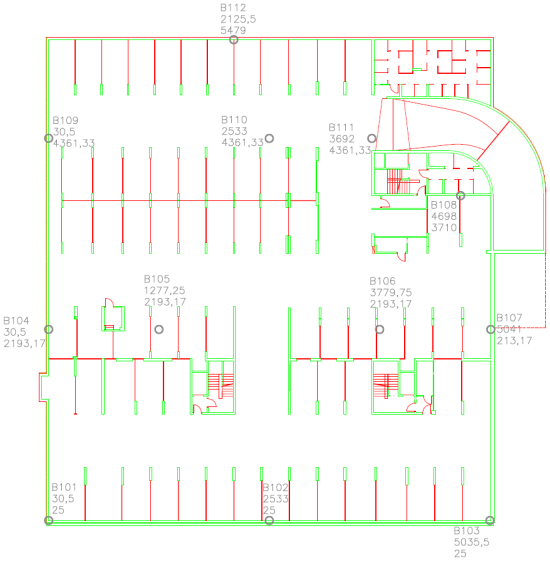
\includegraphics[width=0.9\textwidth]{beacon_-1.png}
\caption{Beacony piętro -1}
\end{center}
\end{figure}

\section{Testy i ich wyniki}
\begin{figure}[htb!p]
\begin{center}
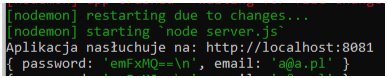
\includegraphics[width=0.9\textwidth]{Przechwytywanie.png}
\caption{Odbiór danych logowania w body}
\end{center}
\end{figure}

\begin{figure}[htb!p]
\begin{center}
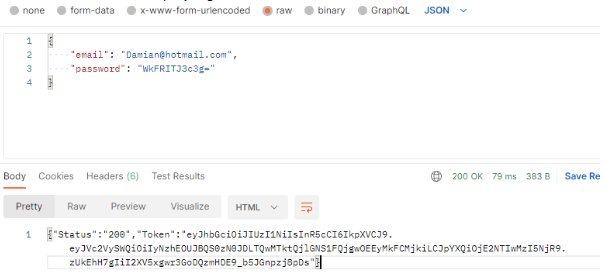
\includegraphics[width=0.9\textwidth]{Przechwytywanie1.png}
\caption{Postman - Odbiór tokena przy logowaniu}
\end{center}
\end{figure}

\section{Podsumowanie i bilans}
Podsumowanie:
\newline

Założenia projektu zawarte w wymaganiach funkcjonalnych zostały wypełnione min.
\begin{itemize}
\item Komunikacja między czujnikami zajętości miejsca a serwerem Ms Sql;
\item Aplikacja webowa,system logowania, system zarządzania;
\item Aplikacja mobilna, rejestracja, logowanie, wyświetlanie ilości wolnych miejsc,\\generowanie QR kodu na podstawie ID użytkownika, zapis bieżącej lokalizacji\\użytkownika, system nawigacji wew. budynkowej na podstawie sygnałów beacon;
\item System sygnalizacji na parkingu.
\end{itemize}
Bilans:
\newline

Początkowe założenia projektu zawierały system nawigowania do najbliższego wolnego miejsca parkingowego. Po dokładnej analizie tej funkcjonalności doszliśmy do wniosku\\że rezygnujemy z tego systemu ze względu na czynnik ludzki (nie zmusimy człowieka do\\zaparkowania w wyznaczonym miejscu jeśli wcześniej będą wolne miejsca).
\newline

Po przeanalizowaniu potrzeb użytkowników w późniejszej fazie projektu,  zdecydowaliśmy się na wprowadzenie systemu zapamiętywania lokalizacji zaparkowanego samochodu oraz\\późniejszej nawigacji do pojazdu.
\newline

 Pozostałe założenia projektu zostały wykonane w całości.

\end{document}